% Options for packages loaded elsewhere
\PassOptionsToPackage{unicode}{hyperref}
\PassOptionsToPackage{hyphens}{url}
%
\documentclass[
]{book}
\usepackage{amsmath,amssymb}
\usepackage{lmodern}
\usepackage{iftex}
\ifPDFTeX
  \usepackage[T1]{fontenc}
  \usepackage[utf8]{inputenc}
  \usepackage{textcomp} % provide euro and other symbols
\else % if luatex or xetex
  \usepackage{unicode-math}
  \defaultfontfeatures{Scale=MatchLowercase}
  \defaultfontfeatures[\rmfamily]{Ligatures=TeX,Scale=1}
\fi
% Use upquote if available, for straight quotes in verbatim environments
\IfFileExists{upquote.sty}{\usepackage{upquote}}{}
\IfFileExists{microtype.sty}{% use microtype if available
  \usepackage[]{microtype}
  \UseMicrotypeSet[protrusion]{basicmath} % disable protrusion for tt fonts
}{}
\makeatletter
\@ifundefined{KOMAClassName}{% if non-KOMA class
  \IfFileExists{parskip.sty}{%
    \usepackage{parskip}
  }{% else
    \setlength{\parindent}{0pt}
    \setlength{\parskip}{6pt plus 2pt minus 1pt}}
}{% if KOMA class
  \KOMAoptions{parskip=half}}
\makeatother
\usepackage{xcolor}
\usepackage{color}
\usepackage{fancyvrb}
\newcommand{\VerbBar}{|}
\newcommand{\VERB}{\Verb[commandchars=\\\{\}]}
\DefineVerbatimEnvironment{Highlighting}{Verbatim}{commandchars=\\\{\}}
% Add ',fontsize=\small' for more characters per line
\usepackage{framed}
\definecolor{shadecolor}{RGB}{248,248,248}
\newenvironment{Shaded}{\begin{snugshade}}{\end{snugshade}}
\newcommand{\AlertTok}[1]{\textcolor[rgb]{0.94,0.16,0.16}{#1}}
\newcommand{\AnnotationTok}[1]{\textcolor[rgb]{0.56,0.35,0.01}{\textbf{\textit{#1}}}}
\newcommand{\AttributeTok}[1]{\textcolor[rgb]{0.77,0.63,0.00}{#1}}
\newcommand{\BaseNTok}[1]{\textcolor[rgb]{0.00,0.00,0.81}{#1}}
\newcommand{\BuiltInTok}[1]{#1}
\newcommand{\CharTok}[1]{\textcolor[rgb]{0.31,0.60,0.02}{#1}}
\newcommand{\CommentTok}[1]{\textcolor[rgb]{0.56,0.35,0.01}{\textit{#1}}}
\newcommand{\CommentVarTok}[1]{\textcolor[rgb]{0.56,0.35,0.01}{\textbf{\textit{#1}}}}
\newcommand{\ConstantTok}[1]{\textcolor[rgb]{0.00,0.00,0.00}{#1}}
\newcommand{\ControlFlowTok}[1]{\textcolor[rgb]{0.13,0.29,0.53}{\textbf{#1}}}
\newcommand{\DataTypeTok}[1]{\textcolor[rgb]{0.13,0.29,0.53}{#1}}
\newcommand{\DecValTok}[1]{\textcolor[rgb]{0.00,0.00,0.81}{#1}}
\newcommand{\DocumentationTok}[1]{\textcolor[rgb]{0.56,0.35,0.01}{\textbf{\textit{#1}}}}
\newcommand{\ErrorTok}[1]{\textcolor[rgb]{0.64,0.00,0.00}{\textbf{#1}}}
\newcommand{\ExtensionTok}[1]{#1}
\newcommand{\FloatTok}[1]{\textcolor[rgb]{0.00,0.00,0.81}{#1}}
\newcommand{\FunctionTok}[1]{\textcolor[rgb]{0.00,0.00,0.00}{#1}}
\newcommand{\ImportTok}[1]{#1}
\newcommand{\InformationTok}[1]{\textcolor[rgb]{0.56,0.35,0.01}{\textbf{\textit{#1}}}}
\newcommand{\KeywordTok}[1]{\textcolor[rgb]{0.13,0.29,0.53}{\textbf{#1}}}
\newcommand{\NormalTok}[1]{#1}
\newcommand{\OperatorTok}[1]{\textcolor[rgb]{0.81,0.36,0.00}{\textbf{#1}}}
\newcommand{\OtherTok}[1]{\textcolor[rgb]{0.56,0.35,0.01}{#1}}
\newcommand{\PreprocessorTok}[1]{\textcolor[rgb]{0.56,0.35,0.01}{\textit{#1}}}
\newcommand{\RegionMarkerTok}[1]{#1}
\newcommand{\SpecialCharTok}[1]{\textcolor[rgb]{0.00,0.00,0.00}{#1}}
\newcommand{\SpecialStringTok}[1]{\textcolor[rgb]{0.31,0.60,0.02}{#1}}
\newcommand{\StringTok}[1]{\textcolor[rgb]{0.31,0.60,0.02}{#1}}
\newcommand{\VariableTok}[1]{\textcolor[rgb]{0.00,0.00,0.00}{#1}}
\newcommand{\VerbatimStringTok}[1]{\textcolor[rgb]{0.31,0.60,0.02}{#1}}
\newcommand{\WarningTok}[1]{\textcolor[rgb]{0.56,0.35,0.01}{\textbf{\textit{#1}}}}
\usepackage{longtable,booktabs,array}
\usepackage{calc} % for calculating minipage widths
% Correct order of tables after \paragraph or \subparagraph
\usepackage{etoolbox}
\makeatletter
\patchcmd\longtable{\par}{\if@noskipsec\mbox{}\fi\par}{}{}
\makeatother
% Allow footnotes in longtable head/foot
\IfFileExists{footnotehyper.sty}{\usepackage{footnotehyper}}{\usepackage{footnote}}
\makesavenoteenv{longtable}
\usepackage{graphicx}
\makeatletter
\def\maxwidth{\ifdim\Gin@nat@width>\linewidth\linewidth\else\Gin@nat@width\fi}
\def\maxheight{\ifdim\Gin@nat@height>\textheight\textheight\else\Gin@nat@height\fi}
\makeatother
% Scale images if necessary, so that they will not overflow the page
% margins by default, and it is still possible to overwrite the defaults
% using explicit options in \includegraphics[width, height, ...]{}
\setkeys{Gin}{width=\maxwidth,height=\maxheight,keepaspectratio}
% Set default figure placement to htbp
\makeatletter
\def\fps@figure{htbp}
\makeatother
\setlength{\emergencystretch}{3em} % prevent overfull lines
\providecommand{\tightlist}{%
  \setlength{\itemsep}{0pt}\setlength{\parskip}{0pt}}
\setcounter{secnumdepth}{5}
\usepackage{booktabs}
\usepackage{amsthm, graphicx, mathtools, amssymb, amsmath}
\makeatletter
\def\thm@space@setup{%
  \thm@preskip=8pt plus 2pt minus 4pt
  \thm@postskip=\thm@preskip
}
\makeatother

\newtheorem*{adamCitation}{Citation}
\newtheorem*{remark}{Remark}
\newtheorem*{definition}{Definition}
\newtheorem*{task}{Task}
\newtheorem*{solution}{Solution}
\DeclareMathOperator\Arg{Arg}
\usepackage{booktabs}
\usepackage{longtable}
\usepackage{array}
\usepackage{multirow}
\usepackage{wrapfig}
\usepackage{float}
\usepackage{colortbl}
\usepackage{pdflscape}
\usepackage{tabu}
\usepackage{threeparttable}
\usepackage{threeparttablex}
\usepackage[normalem]{ulem}
\usepackage{makecell}
\usepackage{xcolor}
\ifLuaTeX
  \usepackage{selnolig}  % disable illegal ligatures
\fi
\usepackage[]{natbib}
\bibliographystyle{elsarticle-harv}
\IfFileExists{bookmark.sty}{\usepackage{bookmark}}{\usepackage{hyperref}}
\IfFileExists{xurl.sty}{\usepackage{xurl}}{} % add URL line breaks if available
\urlstyle{same} % disable monospaced font for URLs
\hypersetup{
  pdftitle={Time Series Analysis and Forecasting with Complex Dynamic Models},
  pdfauthor={Sergey Svetunkov and Ivan Svetunkov},
  hidelinks,
  pdfcreator={LaTeX via pandoc}}

\title{Time Series Analysis and Forecasting with Complex Dynamic Models}
\author{Sergey Svetunkov and Ivan Svetunkov}
\date{2022-11-29}

\begin{document}
\maketitle

{
\setcounter{tocdepth}{1}
\tableofcontents
}
\hypertarget{introduction}{%
\chapter*{Introduction}\label{introduction}}
\addcontentsline{toc}{chapter}{Introduction}

The theory of complex variables functions is actively used in a variety of disciplines, including modern physics and engineering sciences. It is relatively easy to describe the complex phenomena that are studied in these areas of science using the models and methods of this branch of mathematics. Social sciences, being much more complicated due to the unpredictability of human behaviour, tend to use simpler instruments for modelling complex processes (references). For example, there are only few scientific publications in which methods and models of the theory of complex variables functions are used in economics, and they typically use that instrument for diagnostics or statistical tests (references) rather than proper modelling.

In 2012, Springer published the monograph ``Complex-valued Modeling in Economics and Finance'' (Svetunkov, 2012), which presented the theory and methodology of modelling using complex variables in economics. Svetunkov (2012) have summarised the main principles of using complex variables in economics and discussed how to estimate some of those models. While, this was the first monograph that discussed the topic, the first paper in this direction was Ben Tamari (1997). The author first introduced Wealth as a complex variable consisting of Output (real part) and Money (imaginary part) and showed how, even with such an elementary representation, interesting new results can be obtained in the area of economics. Unfortunately, this work has gone unnoticed in scientific world. We became aware of this work only in 2016, when Ben Tamari had kindly sent Sergey Svetunkov his paper.

Since 2012, there has been some development in the area of modelling using complex variables, notably a paper by Svetunkov \& Kourentzes (2022) on Complex Exponential Smoothing and Kourentez et al.~(2019) on an error measure based on the idea of complex numbers. Up until now, the modelling with complex variables has been mainly picked up by academics working in the areas of forecasting and engineering. The latter group has been using complex autoregressions for a couple of decades, modelling and predicting signals. The former group has only started using the principles described in Svetunkov (2012). In other disciplines, complex variables are not used directly for model building. The probable reason for this is the lack of the communication between the disciplines and the inherited inertia of academia.

In a try to speed up the adoption of the new instrument, we have written this monograph, summarising the research that has been done in the area of dynamic models since 2012. We should clarify that the term ``dynamic model'' used in this monograph refers to models that have a structure that changes over time. The classical example of such a model is ARIMA (AutoRegression Integrated with Moving Average by Box \& Jenkins, 1976), which allows producing forecasts for a variety of processes based on the existing historical time series. Another example is a multivariate version of ARMA, Vector ARMA or VARMA, which allows modelling the dynamics of several related processes simultaneously. For instance, in business and economics, these models are used for prices, demand forecasting and for capturing complex interactions between macroeconomic indicators over time.
However, all autoregression models that exist today use real variables. In this monograph we will discuss their complex-valued counterparts, namely complex ARIMA and complex VARMA, and study their properties, showing how to identify their orders and how to estimate these models in practice. But before rushing into the discussion, we will explain the basics of random complex variables and complex-valued statistics, which has been developed in signal processing literature, but has not been used to its full potential.

Chapter 1 discusses the theory of random complex variables, conventional and complex-valued statistics, the complex least squares method, maximum likelihood and complex autocorrelation and partial autocorrelation functions. In Chapter 2, we will move to the discussion of simple dynamic model -- complex AR, starting from its properties and slowly moving to its identification and estimation and then to forecasting. After that, in Chapter 3, we will move towards complex MA, again discussing its properties and how one can apply it in practice. The two parts will be united in a cARIMA model in Chapter 4, where we will also discuss seasonal counterpart of the model. Finally, we will move to vector models in Chapter 5, introducing cVAR, cVMA and cVARMA, showing their advantages in comparison with the conventional real valued models. All of this will be supported by examples in R, which will rely heavily on the package ``complex'', developed especially for this monograph. This means that anyone can then use the proposed models for purposes of time series analysis and forecasting.
This work was partially supported by the Russian Foundation for Basic Research (grant No.~19-010-00610\textbackslash19 ``Theory, methods and methodologies of forecasting economic development by autoregression models of complex variables''). Thanks to this support, it became possible to carry out this research in general, forming a new scientific direction in statistical modelling and short-term forecasting.

The authors are grateful to those young scientists of St.~Petersburg Polytechnic University of Peter the Great, who participated in this study, patiently testing the author's hypotheses. They helped forming the theory behind the models discussed in this monograph. We are pleased to mention their names: Evgeny Goltsev, Nikolai Pitukhin, Victoria Matskevich, Yulia Selivanova, Galina Siruk and Nazira Shaikhleeva.

this monograph relies heavily on the \texttt{complex} package for R. Many of the examples in R will use functions from this package, so make sure to install it before running any R code \citep{R-complex}:

\begin{Shaded}
\begin{Highlighting}[]
\FunctionTok{install.packages}\NormalTok{(}\StringTok{"complex"}\NormalTok{)}
\end{Highlighting}
\end{Shaded}

\hypertarget{intro}{%
\chapter{Introduction to complex random variables}\label{intro}}

\hypertarget{theoryOfComplexNumbers}{%
\section{Theory of complex numbers}\label{theoryOfComplexNumbers}}

This section sets out the basic concepts of the Theory of Complex Variables Functions (TCVF) with some historical overlook of the idea of complex numbers. Hopefully, this will help in understanding the main idea that we will use extensively in the following chapters.

The theory of complex numbers started in 1572 in the small Italian town of Kura. It was in this place and precisely in this year that the manuscript of an Italian mathematician Rafael Bombelli was published. The book was called Algebra. Rafael Bombelli showed in it how to solve the following cubic equation:
\begin{equation}
    x^3 = 15x + 4 .
    \label{eq:BombelliEquation}
\end{equation}
The root of cubic equations at that time was calculated using the formula of Scipione del Ferro. With regards to the task at hand, finding the root should have been carried out as follows:
\begin{equation}
    \begin{aligned}
    x = & \sqrt[3]{\frac{4}{2}+\sqrt{\left(\frac{4}{2}\right)^2 - \left(\frac{15}{3}\right)^3}} + \sqrt[3]{\frac{4}{2}-\sqrt{\left(\frac{4}{2}\right)^2 - \left(\frac{15}{3}\right)^3}} = \\
        & \sqrt[3]{2+\sqrt{-121}} + \sqrt[3]{2-\sqrt{-121}} .
    \end{aligned}
    \label{eq:BombelliSolution}
\end{equation}
As can be seen from equation \eqref{eq:BombelliSolution}, there are several square roots, and it follows directly from the right hand side of this equation that to calculate the roots of equation \eqref{eq:BombelliEquation}, we need to extract the square root from the negative number, -121. This means that it will not be possible to find a solution to this equation in the domain of real numbers.

This does not mean that equation \eqref{eq:BombelliEquation} does not have a solution. If you represent the problem graphically on a plane then it is easy to see that there is one. But it is impossible to find it arithmetically using the Scipione del Ferro formula, because there is a negative number in the expression on the right-hand side of \eqref{eq:BombelliSolution}, and back then, mathematicians were sure that the square root of a negative number does not exist.

The mathematicians of that time struggled to solve this problem, and Rafael Bombelli suggested to ignore the negative sign in the expression (Bombelli, 12). After all, the number -121 can be represented as a product of two numbers: -1 and 121. Then the square root of this number can be written as \(\sqrt{-1} \times 11\). So, formula \eqref{eq:BombelliSolution} becomes:
\begin{equation}
    x = \sqrt[3]{2+11\sqrt{-1}} + \sqrt[3]{2-11\sqrt{-1}} .
    \label{eq:BombelliSolutionSqrt}
\end{equation}
Now it is possible to get a solution of the problem, and the root of the cubic equation is \(x = 4\).

For a long time, Bombelli's approach was considered by scientists as a convenient mathematical trick. And the square root of minus one was called ``magic unit'', ``vanishing unit'', etc. Finally, the term ``imaginary unit'' was established by René Descartes in 1637 and any number multiplied by the imaginary unit would be called ``imaginary number''. Merging a real number with an imaginary number gives another number, which can be considered as a more general to the two, which is called ``complex''. It can be written as:
\begin{equation}
    z = x+iy ,
    \label{eq:complexNumber}
\end{equation}
where \(x\) is the real part, \(iy\) is the imaginary part of a complex number, \(x\) and \(y\) are real numbers and \(i\) is the imaginary unit that satisfies the equality:
\begin{equation}
    i^2 = -1 .
    \label{eq:imaginaryUnit}
\end{equation}

With complex numbers, one can perform almost all the same operations as with the real ones. However, taking into account the properties of the imaginary unit, these operations can lead to results that are not common in the domain of real numbers.

The main problem that analysts face when trying to understand a complex number is the complexity of the interpretation of the imaginary part. The main question in this case can be formulated as: Where do imaginary numbers appear in practice? And what is the practical meaning of an imaginary unit? We have heard questions like that many times, and while they are valid, we think that they do not have appropriate answers and divert the analysts from what the modelling with complex variables brings.

We argue that the imaginary unit does not have any practical meaning: neither in economics, nor in sociology, nor in engineering, nor in physics. The imaginary unit is a mathematical rule, and that is all. It is a mathematical abstract that has useful properties. A number \(\sqrt{2}\) or \(\ln 3\) do not have practical meaning either, but they are useful for modelling purposes and solving applied problems in a variety of disciplines. Similarly, an imaginary unit is convenient for solving a whole class of problems in different areas of application. With the help of the rules specified by conditions \eqref{eq:complexNumber} and \eqref{eq:imaginaryUnit}, it is possible to use new mathematical operations, obtain new mathematical results, and create new mathematical models.

Imaginary and complex numbers are mathematical instruments that can help in describing a real-life phenomenon. If a researcher decides to use complex variables for real processes modelling, they will need to predefine the rules according to which one component of a complex process is attributed to the real part, and another one is attributed to the imaginary part of the complex variable. These rules might seem arbitrary, because there is no ``true'' recipe, according to which the assignment to complex variable parts should be done. The main motivation for them is the efficiency of modelling (such as goodness of fit or forecasting accuracy) and nothing else.

In order to better understand how the modelling with complex variables can be done, we need to better understand how complex variables can be represented and interpreted. A real number represents visually a certain segment on the numerical axis, which has a zero point and a multitude of values from minus infinity to infinity. Any real number is characterized by the distance from zero to the value of that number. Negative numbers are located to the left of zero, while the positive ones are located to the right of it.

A complex number consists of two parts, which can be visualised on the plane with two perpendicular axes, where the real numbers are marked on the horizontal line, and the imaginary ones are on the vertical one. This is shown visually in Figure \ref{fig:complexPlane} with a complex number \(z=x+iy\).

\begin{figure}
\centering
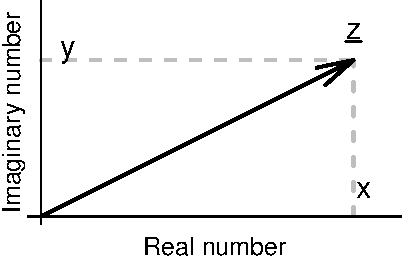
\includegraphics{Svetunkov---Svetunkov---Complex-Dynamic-Models_files/figure-latex/complexPlane-1.pdf}
\caption{\label{fig:complexPlane}Visual presentation of a complex number on the complex plane.}
\end{figure}

Any point lying on the complex plane in Figure \ref{fig:complexPlane} characterises a complex number, even if that point lies on the axis of real numbers. In that specific case, we would be talking about a complex number with a zero imaginary part, i.e.~\(z=x+i0\).

Given that complex numbers can be represented on a plane (in so called Cartesian coordinates), the number \eqref{eq:complexNumber} can be represented in a form of a vector that starts in the origin of coordinates and ends at the point (x, y). Then any complex number can be represented in form of polar coordinates using the magnitude of the vector and its polar angle:
\begin{equation}
    z = x+iy = r (\cos \phi + i \sin \phi),
    \label{eq:complexNumberTrigonometric}
\end{equation}
where \(r=|z|\) is the magnitude, which is calculated as a Euclidean distance from the origin to the point (x, y) on the plane:
\begin{equation}
    r = \sqrt{x^2 + y^2},
    \label{eq:complexNumberMagnitude}
\end{equation}
and \(\phi=\Arg(z)\) is the angle, which equals to:
\begin{equation}
    \phi = \arctan \frac{y}{x} + 2 \pi l,
    \label{eq:complexNumberAngle}
\end{equation}
where \(l\) is an integer number. While depending on a task, \(l\) can be set to a positive, a negative number, or a zero, for convenience, we will restrict it to \(l=0\), because all the other values will not be useful for the inference in following chapters. The polar angle is sometimes referred to as the argument of a complex number.

Using the magnitude and the polar angle, we can also represent any complex number in the exponential form, which was first proposed in 1748 by Euler, in his book ``Introduction to the Infinitesimal Analysis'' \textbf{(Euler, 1961, pp.~118-119)}, which:
\begin{equation}
    z = r e^{i \phi} ,
    \label{eq:complexNumberExponential}
\end{equation}
where \(e\) is the Euler's constant. Equation \eqref{eq:complexNumberExponential} is nowadays also called ``Euler's form''. Comparing @ref\{eq:complexNumberTrigonometric\} with @ref\{eq:complexNumberExponential\}, we can conclude that:
\begin{equation}
    e^{i \phi} = \cos \phi + i \sin \phi ,
    \label{eq:EulerFormula}
\end{equation}
which gives the connection between the linear, trigonometric and exponential forms of a complex number. In the exponential form \eqref{eq:complexNumberExponential}, a positive real number has \(\phi=0\), while a negative one has \(\phi=\pi\), and all imaginary numbers have an angle dividable by \(\frac{\pi}{2}\). So, for example:
\begin{equation*}
    \begin{aligned}
    41 = & 41 e^{i 0} \\
    i41 = & 41 e^{i \frac{\pi}{2}} \\
    -41 = & 41 e^{i \pi} \\
    -i41 = & 41 e^{i \frac{3 \pi}{2}}
    \end{aligned}
\end{equation*}
In fact, multiplication of any complex number by the imaginary unit implies the rotation of complex vector by \(\frac{\pi}{2}\), as shown in Figure \ref{fig:complexPlaneMultiplication}, where a complex number \(z_1 = x_1 + i y_1\) becomes \(z_2 = z_1 \times i = x_2 + i y_2\) etc.

\begin{figure}
\centering
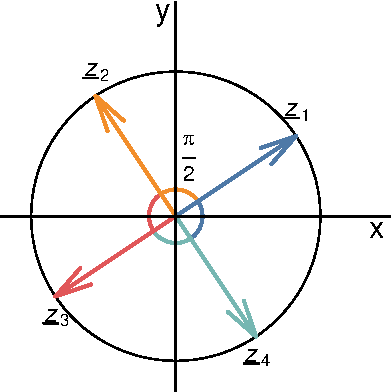
\includegraphics{Svetunkov---Svetunkov---Complex-Dynamic-Models_files/figure-latex/complexPlaneMultiplication-1.pdf}
\caption{\label{fig:complexPlaneMultiplication}Multiplication of a complex number by \(i\) implies the rotation of it by \(\frac{\pi}{2}\).}
\end{figure}

In a way, any mathematical operation with a complex number implies a change in magnitude and angle of the number, while the multiplication and division by a number with non-zero imaginary part will always lead to the rotation of the vector. Operations of addition and subtraction are simpler in the linear form:
\begin{equation*}
    z_3 = z_1 + z_2 = x_1 + x_2 + i (y_1 + y_2) ,
\end{equation*}
while operations of multiplication and division are easier to do in either exponential or trigonometric forms of complex numbers:
\begin{equation*}
    z_3 = z_1 \times z_2 = r_1 r_2 e^{i \phi_1 + \phi_2} 
\end{equation*}
or:
\begin{equation*}
    z_3 = r_1 r_2 \left(\cos (\phi_1 + \phi_2) + i \sin (\phi_1 + \phi_2) \right) .
\end{equation*}

Furthermore, given that any complex number can be represented in the exponential form \eqref{eq:complexNumberExponential}, it can also be visualised on a polar coordinates plane, where the magnitude is marked on the x-axis, and the polar angle is marked on the y-axis. This is shown visually in Figure \ref{fig:complexPlanePolar}.

\begin{figure}
\centering
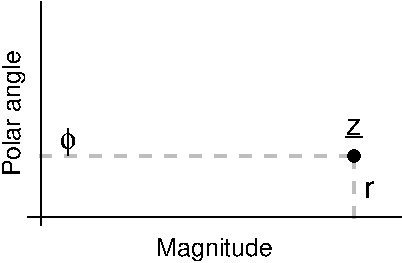
\includegraphics{Svetunkov---Svetunkov---Complex-Dynamic-Models_files/figure-latex/complexPlanePolar-1.pdf}
\caption{\label{fig:complexPlanePolar}Visual presentation of a complex number in the polar coordinates.}
\end{figure}

The usefulness of the polar coordinates presentation becomes apparent when a set of complex numbers is considered, because then in some cases it becomes possible to see some relations that are not obvious on the Cartesian plane. Figure \ref{fig:complexCartesianvsPolar} shows an example of a set of complex random numbers, for which the real and imaginary parts do not seem to have any obvious linear relation, but the magnitude and the angle have a negative relation.

\begin{figure}
\centering
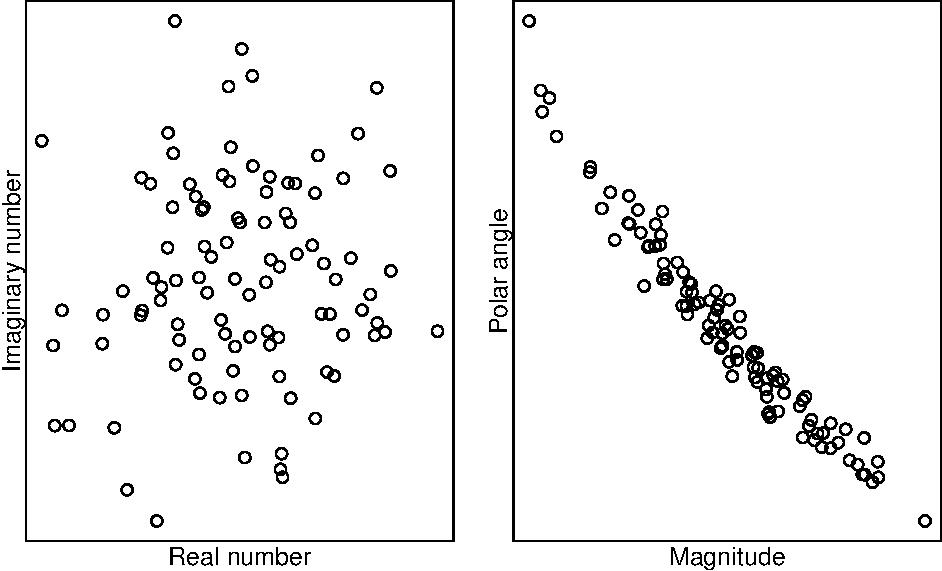
\includegraphics{Svetunkov---Svetunkov---Complex-Dynamic-Models_files/figure-latex/complexCartesianvsPolar-1.pdf}
\caption{\label{fig:complexCartesianvsPolar}Visualisation of a set of complex numbers on Cartesian and on polar coordinates planes.}
\end{figure}

In this case, modelling can be done in the exponential form of complex numbers, which might allow capturing complicated non-linear relations between variables.

When it comes to comparing complex numbers, mathematically we will say that two complex numbers \(z_1 = x_1 + i y_1\) and \(z_2 = x_2 + i y_2\) are equal to each other if and only if their real and imaginary parts are equal:
\begin{equation*}
    z_1 = z_2 \iff \left \lbrace
    \begin{aligned}
        & x_1 = x_2 \\
        & y_1 = y_2
    \end{aligned}
    \right. ,
\end{equation*}
which is equivalent to saying that their magnitudes and polar angles are equal:
\begin{equation*}
    z_1 = z_2 \iff \left \lbrace
    \begin{aligned}
        & |z_1| = |z_2| \\
        & \Arg(z_1) = \Arg(z_2)
    \end{aligned}
    \right. .
\end{equation*}

Unfortunately, given that complex numbers are two dimensional, it is not possible to say in general whether one number is greater or less than the other. However, we could use magnitude to compare complex numbers, to say which one lies further away from the origin than the other. In that case, the number with a larger magnitude could be considered as a greater than the one with the smaller magnitude. While we could compare the polar angles as well, they only give us information about rotation of a complex number and thus do not give any meaningful information about the comparison of numbers. So, two complex numbers in Figure \ref{fig:complexPlaneCircle} would have the same magnitude, but will have different angles, and it is not possible to say whether one number is greater than the other in this case. In order to conclude that, we would need to devise additional criteria for comparison of numbers (e.g.~positive numbers are ``better'' than the negative ones, thus \(\phi_1=\pi\) and \(\phi_1=-\pi\) is ``worse'' than \(\phi_2=0\)).

\begin{figure}
\centering
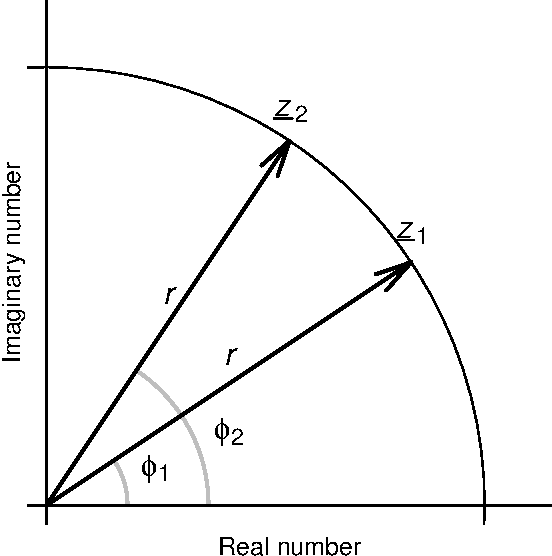
\includegraphics{Svetunkov---Svetunkov---Complex-Dynamic-Models_files/figure-latex/complexPlaneCircle-1.pdf}
\caption{\label{fig:complexPlaneCircle}Comparison of two complex numbers \(z_1\) and \(z_2\) that have the same magnitude \(r\), but different angles \(\phi_1\) and \(\phi_2\).}
\end{figure}

Continuing the discussion of different forms of a complex number, its magnitude can be represented in exponential form:
\begin{equation*}
    r = e^{\ln(r)},
\end{equation*}
where \(\ln\) is the natural logarithm. This can then be used to rewrite the exponential form of a complex number as:
\begin{equation}
    z = e^{\ln r + i \phi} ,
    \label{eq:complexNumberExponentialAll}
\end{equation}
And this form allows calculating logarithms of a complex number:
\begin{equation*}
    \ln z = \ln \left(e^{\ln r + i \phi} \right) = \ln r + i \phi .
\end{equation*}
This operation will become useful when we discuss transformations of complex-valued functions, but it also shows that a logarithm of a negative real number is a complex number, because in that case \(\phi=\pi\). This demonstrates that the field of complex numbers is complete: any mathematical operation of a complex number will give another complex number.

One of the important definitions in theory of complex numbers is the conjugate complex number. It is the number, for which the imaginary part has the sign opposite to the one of the original variable. For example, the conjugate of the complex variable \(z = x+ iy\) is \(\tilde{z} = x- iy\). These numbers are useful because the multiplication of a complex number by its conjugate gives a real number:
\begin{equation}
    z \times \tilde{z} = (x+ iy) (x- iy) = x^2 + y^2 ,
    \label{eq:complexNumberConjugateMulti}
\end{equation}
which is the square of the magnitude \eqref{eq:complexNumberMagnitude} of both complex variables \(z\) and \(\tilde{z}\).

Finally, given that any complex number can be represented visually in a form of a vector, we can write it mathematically either like vector:
\begin{equation}
    \begin{pmatrix} x \\ y \end{pmatrix}
    \label{eq:complexNumberVectors}
\end{equation}
or like a matrix:
\begin{equation}
    \begin{pmatrix} x & -y \\ y & x \end{pmatrix} .
    \label{eq:complexNumberMatrix}
\end{equation}
In the latter case, the real number can be represented as a diagonal matrix, while the imaginary one is the matrix with zero diagonal:
\begin{equation*}
    \begin{aligned}
        & \begin{pmatrix} x & 0 \\ 0 & x \end{pmatrix} \\
        & \begin{pmatrix} 0 & -y \\ y & 0 \end{pmatrix}
    \end{aligned} .
\end{equation*}
All the mathematical operations done with the vector and matrix representations would correspond to the ones for the conventional complex numbers. Furthermore, the multiplication by the transpose of the original object in both of these cases is equivalent to the multiplication by the conjugate value \eqref{eq:complexNumberConjugateMulti}. For the vector:
\begin{equation}
    \begin{pmatrix} x & y \end{pmatrix} \times \begin{pmatrix} x \\ y \end{pmatrix} = \begin{pmatrix} x^2 + y^2 \end{pmatrix}
    \label{eq:complexNumberVectorsMulti}
\end{equation}
and for the matrix:
\begin{equation}
    \begin{pmatrix} x & -y \\ y & x \end{pmatrix} \times \begin{pmatrix} x & y \\ -y & x \end{pmatrix} = 
    \begin{pmatrix} x^2 + y^2 & 0 \\ 0 & x^2 + y^2 \end{pmatrix}.
    \label{eq:complexNumberMatrixMulti}
\end{equation}
These representations become especially useful when we work with complex variables to construct complex models.

\hypertarget{complexVariable}{%
\subsection{Complex variables}\label{complexVariable}}

Similarly to any other variable, complex variable is a place holder for values, with the difference that it represents two parts of a number instead of one. Given the properties of complex numbers discussed in the previous section, any complex variable can be represented in linear, trigonometric and exponential forms. But in addition, it can also be represented in the form of a set of equations, i.e.~if \(y_r + i y_i = 3+2i\) then:
\begin{equation}
    \begin{aligned}
        y_r = & 3 \\
        y_i = & 2
    \end{aligned} ,
    \label{eq:complexVariablesSystem}
\end{equation}
where the subscript \(r\) or \(i\) refers to respectively the real or imaginary parts of the complex number. In fact, any function of a complex variable can be represented as system of two equations, so that for a function
\begin{equation}
    y_{r} + i y_{i} = f(x_r+ix_i)
    \label{eq:complexFunction}
\end{equation}
we have:
\begin{equation}
    \begin{aligned}
        y_r = & \mathcal{R}(f(x_r+ix_i)) \\
        y_i = & \mathcal{I}(f(x_r+ix_i))
    \end{aligned} ,
    \label{eq:complexFunctionSystem}
\end{equation}
where \(\mathcal{R}()\) and \(\mathcal{I}()\) are respectively the real and the imaginary parts of a resulting complex variable. For example, a simple linear function:
\begin{equation*}
    y_r + i y_i = a_{0,r} + i a_{0,i} + (a_{1,r} + i a_{1,i}) (x_{1,r} + i x_{1,i}),
\end{equation*}
which can be written after opening the brackets and regrouping elements as:
\begin{equation*}
    y_r + i y_i = a_{0,r} + a_{1,r} x_{1,r} - a_{1,i} x_{1,i} + i \left( a_{0,i} + a_{1,i} x_{1,r} + a_{1,r} x_{1,i} \right)
\end{equation*}
and is equivalent to the system of the following two equations:
\begin{equation*}
    \begin{aligned}
        y_r = & a_{0,r} + a_{1,r} x_{1,r} - a_{1,i} x_{1,i} \\
        y_i = & a_{0,i} + a_{1,i} x_{1,r} + a_{1,r} x_{1,i}
    \end{aligned} .
\end{equation*}
Given the vector and matrix representation of complex variables, the same linear function can be written as:
\begin{equation*}
    \begin{pmatrix} y_r \\ y_i \end{pmatrix} = \begin{pmatrix} a_{0,r} \\ a_{0,i} \end{pmatrix} + \begin{pmatrix} a_{1,r} & -a_{1,i} \\ a_{1,i} & a_{1,r} \end{pmatrix} \begin{pmatrix} x_{1,r} \\ x_{1,i} \end{pmatrix} ,
\end{equation*}
which is convenient in some situations. Presenting the system of equations \eqref{eq:complexFunctionSystem} in the linear form \eqref{eq:complexFunction} is often convenient. In fact, any function of complex variables can be represented as a system of two functions. Even if the real or the imaginary part of the output complex variable \(y_r + i y_i\) is equal to zero, we can still use a system of two equations, where one of the equations becomes just a constraint for the function. For example, if we assume that \(y_i=0\), then the system \eqref{eq:complexFunctionSystem} becomes:
\begin{equation*}
    \begin{aligned}
        & y_r = \mathcal{R}(f(x_r+ix_i)) \\
        & \mathcal{I}(f(x_r+ix_i)) = 0
    \end{aligned} .
\end{equation*}
This property becomes especially useful if one needs to construct a model with linear relations between the input variables \citep[this is discussed in Chapter ??? of][]{Svetunkov2014}.

Given the discussion about the vector and matrix forms of complex numbers, the system of equations \eqref{eq:complexFunctionSystem} can be written as:
\begin{equation}
    \begin{pmatrix} y_r \\ y_i \end{pmatrix} =
    \begin{pmatrix} \mathcal{R}(f(x_r+ix_i)) \\ \mathcal{I}(f(x_r+ix_i)) \end{pmatrix} .
    \label{eq:complexFunctionVectors}
\end{equation}
or:
\begin{equation}
    \begin{pmatrix} \mathcal{R}(f(x_r+ix_i)) & - \mathcal{I}(f(x_r+ix_i)) \\ \mathcal{I}(f(x_r+ix_i)) & \mathcal{R}(f(x_r+ix_i)) \end{pmatrix} .
    \label{eq:complexFunctionMatrix}
\end{equation}
The representations \eqref{eq:complexFunction}, \eqref{eq:complexFunctionSystem}, \eqref{eq:complexFunctionVectors} and \eqref{eq:complexFunctionMatrix} are equivalent and can be used interchangeably depending on the task at hand.

Finally, in terms of definitions, the function \eqref{eq:complexFunction} is often referred to as a ``complex-valued'' function. It maps a certain values of the input variable \(x_r + i x_i\) with a specific value of the output variable \(y_r +i y_i\). If there is only a one-to-one relation between the input and output variables then such function is called ``univalent''. When several different values of the input variable leads to one and the same value of the output variable then the function is called ``multivalent''. An example of the former is the linear function:
\begin{equation*}
    y_r + i y_i = (a_{1,r} + i a_{1,i}) (x_{1,r} + i x_{1,i}),
\end{equation*}
while for the latter, an example is
\begin{equation*}
    y_r + i y_i = (a_{1,r} + i a_{1,i}) (x_{1,r} + i x_{1,i})^2, 
\end{equation*}
where two different input complex numbers (for example \(0 + i\) and \(0-i\)) correspond to the same output number (\(-1 + i0\)). While there are examples of functions like that in the real domain, in the complex one, they appear even more often due to the rotation property discussed in the previous Subsection.

\hypertarget{complexRandomVariable}{%
\section{Complex random variable}\label{complexRandomVariable}}

In statistics, a random variable is a variable, the value of which depends on random events. For example, for the classical coin tossing experiment, \(x\) would be considered as a random variable if it is equal to 1 in case of heads and is equal to zero otherwise. In case of complex random variables (c.r.v.), the logic is similar, but we would typically deal with two-dimensional cases (e.g.~tossing two coins simultaneously). We accept that in some cases, some parts of the c.r.v. might become non-random (e.g.~the real part becomes equal to some fixed number). As such, we would be saying that \(x=x_r+ix_i\) is a complex random variable if at least one part of it follows some distribution. Furthermore, while random variables can be measured in a variety of scales (coin tossing represents the nominal scale), in this monograph we focus the discussion on continuous numerical variables.

As any other random variable, c.r.v. can be characterised by its moments. However, some of its moments differ from the conventional ones for real variables and are based on the properties of complex numbers.

\hypertarget{first-moment}{%
\subsection{First moment}\label{first-moment}}

The first moment of any c.r.v. is relatively straightforward. For the variable \(x=x_r+ix_i\) it is:
\begin{equation}
    \mu = \mathrm{E}(x) = \mathrm{E}(x_r + i x_i) = \mathrm{E}(x_r) + i \mathrm{E}(x_i) = \mu_{r} + i \mu_{i},
    \label{eq:crvMomentFirst}
\end{equation}
due to the law of total expectation and because \(i\) is a constant. In \eqref{eq:crvMomentFirst}, \(\mathrm{E}(.)\) is the expectation of a variable, \(\mu\) is the first moment of a complex variable and \(\mu_{r}\) and \(\mu_{i}\) are the respective real and imaginary parts of the first moment. In sample, this moment can be calculated as:
\begin{equation}
    \hat{\mu} = \hat{\mu}_{r} + i \hat{\mu}_{i} = \frac{1}{n}\sum_{j=1}^n x_{r,j} + i \frac{1}{n}\sum_{j=1}^n x_{i,j},
    \label{eq:crvMomentFirstSample}
\end{equation}
where \(n\) is the sample size and \(\hat{\mu}\) is the estimate of \(\mu\). The properties of the first moment of c.r.v. are similar to the properties of any other random variable. The only thing to note is that the moment can also be represented in a vector or matrix form (see Subsection \ref{complexVariable}):
\begin{equation}
    \begin{pmatrix} \mu_{r} \\ \mu_{i} \end{pmatrix} 
    \label{eq:crvMomentsVector}
\end{equation}
or
\begin{equation}
    \begin{pmatrix} \mu_{r} & - \mu_{i} \\ \mu_{i} & \mu_{r} \end{pmatrix} .
    \label{eq:crvMomentsMatrix}
\end{equation}

In R, the first moment can be obtained via the \texttt{mean()} function from \texttt{stats} package:

\begin{Shaded}
\begin{Highlighting}[]
\CommentTok{\# Create a random variable}
\NormalTok{x }\OtherTok{\textless{}{-}} \FunctionTok{complex}\NormalTok{(}\AttributeTok{real=}\FunctionTok{rnorm}\NormalTok{(}\DecValTok{100}\NormalTok{, }\AttributeTok{mean=}\DecValTok{50}\NormalTok{, }\AttributeTok{sd=}\DecValTok{10}\NormalTok{),}
             \AttributeTok{imaginary=}\FunctionTok{rnorm}\NormalTok{(}\DecValTok{100}\NormalTok{, }\AttributeTok{mean=}\DecValTok{100}\NormalTok{, }\AttributeTok{sd=}\DecValTok{10}\NormalTok{))}
\CommentTok{\# Calculate the first moment}
\FunctionTok{mean}\NormalTok{(x)}
\end{Highlighting}
\end{Shaded}

\begin{verbatim}
## [1] 50.1773+100.657i
\end{verbatim}

\hypertarget{crvSecondMoment}{%
\subsection{Second moment}\label{crvSecondMoment}}

While there are raw moments for c.r.v., here we will focus on the centred ones, i.e.~moments for \(x-\bar{x}\). There are several instruments related to the second moment that could characterise a complex random variable. The first one is called ``variance'' and is based on the multiplication by a conjugate number \citep{reference}. So for the c.r.v. \(x_r + i x_i\) the variance is:
\begin{equation}
    \begin{aligned}
    \sigma_x^2 = & \mathrm{E}((x-\mu) (\tilde{x}-\tilde{\mu})) = \mathrm{E}\left(((x_r-\mu_{r}) + i (x_i-\mu_{i}))((x_r-\mu_{r}) - i (x_i-\mu_{i}))\right) = \\
                & \mathrm{E}((x_r-\mu_{r})^2) +  \mathrm{E}((x_i-\mu_{i})^2)
    \end{aligned}
    \label{eq:crvMomentSecondVariance}
\end{equation}
or taking that the variances of the real and the imaginary parts are \(\sigma_{x_r}^2\) and \(\sigma_{x_i}^2\) respectively:
\begin{equation}
    \sigma_x^2 = \sigma_{x_r}^2 + \sigma_{x_i}^2.
    \label{eq:crvMomentSecondVarianceShort}
\end{equation}
Multiplication by conjugate in \eqref{eq:crvMomentSecondVariance} allows keeping the size of variability for both real and imaginary parts, but at the same time masks the individual contribution of each part in the overall variance and removes the covariance between the parts. The resulting values shows in a way the overall variability of a c.r.v. along a diagonal line as shown in Figure \ref{fig:crvMomentSecondVariance}.

\begin{figure}
\centering
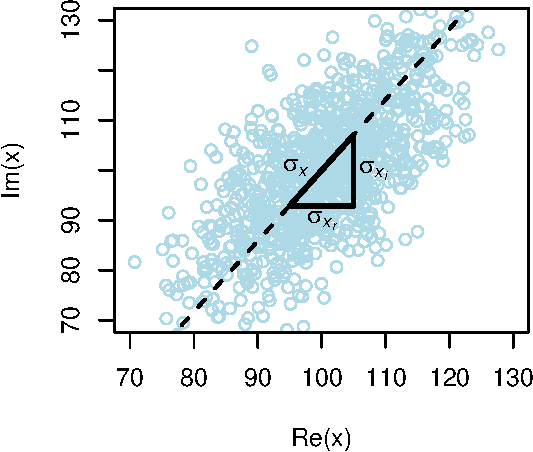
\includegraphics{Svetunkov---Svetunkov---Complex-Dynamic-Models_files/figure-latex/crvMomentSecondVariance-1.pdf}
\caption{\label{fig:crvMomentSecondVariance}Visual representation of variance of a complex random variable.}
\end{figure}

Figure \ref{fig:crvMomentSecondVariance} demonstrates graphically the relation between standard deviations of real, imaginary and the overall variance of a complex variable according to the formula \eqref{eq:crvMomentSecondVarianceShort}.

\citet{Picinbono} note that the moment \eqref{eq:crvMomentSecondVarianceShort} is not sufficient to entirely describe the second order statistics of a c.r.v. This is because it ignores the potential covariance between the parts of a variable and only describes their average variability. Another measure of variability of a complex random variable is the so called ``pseudo-variance'' \citep{reference}, which can be obtained by applying the conventional formula of variance directly to the c.r.v. without the multiplication by conjugate:
\begin{equation}
    \begin{aligned}
    \varsigma_x^2 = & \mathrm{E}(x-\mu^2) = \mathrm{E}\left(((x_r-\mu_{r}) + i (x_i-\mu_{i}))^2\right) = \\
                    & \mathrm{E}((x_r-\mu_{r})^2) - \mathrm{E}((x_i-\mu_{i})^2) + i2 \mathrm{E}((x_r-\mu_{r})(x_i-\mu_{i}))
    \end{aligned}
    \label{eq:crvMomentSecondVariancePseudo}
\end{equation}
or using the notation \(\sigma_{x_r,x_i}\) for covariance between the real and imaginary parts:
\begin{equation}
    \varsigma_x^2 = \sigma_{x_r}^2 - \sigma_{x_i}^2 + i2 \sigma_{x_r,x_i}.
    \label{eq:crvMomentSecondVariancePseudoShort}
\end{equation}
In the literature, the moment \eqref{eq:crvMomentSecondVariancePseudoShort} is called pseudo-variance \citep{reference}, because it does not measure the variability of a variable, but rather gives a different information: it shows whether the real and imaginary variances are similar and what the covariance between them is. If both real and imaginary parts of \eqref{eq:crvMomentSecondVariancePseudoShort} are equal to zero then it is said that the distribution of the complex variable \(x\) is spherical \citep{reference}, i.e.~the variances are similar and the real and imaginary parts are not linearly related. Furthermore, we should point out that while minimising \eqref{eq:crvMomentSecondVarianceShort} implies minimising both variances of the real and imaginary parts of \(x\) (ignoring the covariance between them), minimising \eqref{eq:crvMomentSecondVariancePseudoShort} is not as straightforward. At very least, we could tell that it implies making the distribution of \(x\) closer to the spherical one, but we cannot provide any thorough insight about this.

We should note that both measures can be considered as complex, and the main distinction between them is the multiplication by the same c.r.v or by its conjugate. As such we propose to call them respectively ``conjugate variance'' and ``direct variance''.

In R, the conjugate and direct variances are available in \texttt{cvar()} function of \texttt{complex} package.

\begin{Shaded}
\begin{Highlighting}[]
\CommentTok{\# Create a random variable}
\NormalTok{x }\OtherTok{\textless{}{-}} \FunctionTok{complex}\NormalTok{(}\AttributeTok{real=}\FunctionTok{rnorm}\NormalTok{(}\DecValTok{100}\NormalTok{, }\AttributeTok{mean=}\DecValTok{50}\NormalTok{, }\AttributeTok{sd=}\DecValTok{5}\NormalTok{),}
             \AttributeTok{imaginary=}\FunctionTok{rnorm}\NormalTok{(}\DecValTok{100}\NormalTok{, }\AttributeTok{mean=}\DecValTok{100}\NormalTok{, }\AttributeTok{sd=}\DecValTok{10}\NormalTok{))}
\CommentTok{\# Calculate the conjugate variance}
\FunctionTok{cvar}\NormalTok{(x, }\AttributeTok{kind=}\StringTok{"conjugate"}\NormalTok{) }\SpecialCharTok{|\textgreater{}}
    \FunctionTok{setNames}\NormalTok{(}\StringTok{"Conjugate variance"}\NormalTok{)}
\end{Highlighting}
\end{Shaded}

\begin{verbatim}
## Conjugate variance 
## 118.6764+0i
\end{verbatim}

\begin{Shaded}
\begin{Highlighting}[]
\CommentTok{\# Calculate the direct variance}
\FunctionTok{cvar}\NormalTok{(x, }\AttributeTok{kind=}\StringTok{"direct"}\NormalTok{) }\SpecialCharTok{|\textgreater{}}
    \FunctionTok{setNames}\NormalTok{(}\StringTok{"Direct variance"}\NormalTok{)}
\end{Highlighting}
\end{Shaded}

\begin{verbatim}
##    Direct variance 
## -76.07807+12.9734i
\end{verbatim}

As we see from the output above, the direct variance has the negative real part, which indicates that the imaginary part has higher variance than the real one. The imaginary part of the direct variance shows the double covariance between the real and imaginary parts. Finally, the conjugate variance should be \(5^2 + 10^2 = 125\), but due to small sample (100 observations in the generated random variable above), it will be equal to a number close to it.

Given that any complex variable can be represented in a vector form, the c.r.v. \(x\) can be treated as a bivariate random variable, for which a covariance matrix can be calculated via:
\begin{equation}
    \boldsymbol{\Sigma}_x = \begin{pmatrix} \sigma_{x_r}^2 & \sigma_{x_r, x_i} \\ \sigma_{x_r, x_i} & \sigma_{x_i}^2 \end{pmatrix} .
    \label{eq:crvMomentSecondVarianceMatrix}
\end{equation}
The minimisation of the matrix \eqref{eq:crvMomentSecondVarianceMatrix} does not make sense, but instead it is possible to minimise the determinant of that matrix, which is called ``Generalised Variance'' (GV):
\begin{equation}
    \mathrm{GV} = |\boldsymbol{\Sigma}_x| = \sigma_{x_r}^2 \sigma_{x_i}^2 - \sigma_{x_r, x_i}^2 .
    \label{eq:crvMomentSecondGV}
\end{equation}

In R, this is implemented in \texttt{covar()} function from the \texttt{complex} package:

\begin{Shaded}
\begin{Highlighting}[]
\FunctionTok{covar}\NormalTok{(x)}
\end{Highlighting}
\end{Shaded}

\begin{verbatim}
##           x_r       x_i
## x_r 21.299181  6.486699
## x_i  6.486699 97.377249
\end{verbatim}

The minimisation of GV, as can be seen from the formula \eqref{eq:crvMomentSecondGV}, implies the simultaneous minimisation of variances of real and imaginary parts and maximisation of the square of covariance between them, making the resulting distribution compacter and emphasising the potential relations between the real and imaginary parts of a c.r.v. For our example in R, the GV equals to:

\begin{Shaded}
\begin{Highlighting}[]
\FunctionTok{covar}\NormalTok{(x) }\SpecialCharTok{|\textgreater{}} \FunctionTok{det}\NormalTok{()}
\end{Highlighting}
\end{Shaded}

\begin{verbatim}
## [1] 2031.978
\end{verbatim}

All the three moments discussed in this subsection rely on variances of real and imaginary parts of a c.r.v. and on a covariance between those parts. These moments in turn can be calculated using the conventional formulae, correcting for the potential small sample bias \citep{referenceSBA}:
\begin{equation}
    \begin{aligned}
        \hat{\sigma}_{x_r}^2 = & \frac{1}{n-k} \sum_{j=1}^n (x_{r,j}-\bar{x}_{r,j})^2 \\
        \hat{\sigma}_{x_i}^2 = & \frac{1}{n-k} \sum_{j=1}^n (x_{i,j}-\bar{x}_{i,j})^2 \\
        \hat{\sigma}_{x_r, x_i} = & \frac{1}{n-k} \sum_{j=1}^n (x_{r,j}-\bar{x}_{r,j})(x_{i,j}-\bar{x}_{i,j})^2 ,
    \end{aligned}
    \label{eq:crvMomentSecondSample}
\end{equation}
where \(k\) is the number of estimated parameters in a model.

Finally, similar to the variance it is possible to calculate second moments between two complex random variables \(x = x_r+i x_i\) and \(y = y_r + i y_i\) \citep{Picinbono}. The ``conjugate'' covariance is calculated similarly to \eqref{eq:crvMomentSecondVariance} via the multiplication by conjugate:
\begin{equation}
    \begin{aligned}
    \sigma_{x,y} = & \mathrm{E}((\tilde{x}-\tilde{\mu}_x) (y-\mu_y)) = \\
                   & \mathrm{E}\left(((x_r-\mu_{x,r}) - i (x_i-\mu_{x,i}))((y_r-\mu_{y,r}) + i (y_i-\mu_{y,i}))\right) = \\
                   & \mathrm{E}((x_r-\mu_{x,r})(y_r-\mu_{y,r})) + \mathrm{E}((x_i-\mu_{x,i})(y_i-\mu_{y,i})) + \\
                   & i \left(\mathrm{E}((x_r-\mu_{x,r})(y_i-\mu_{y,i})) - \mathrm{E}((x_i-\mu_{x,i})(y_r-\mu_{y,r}))\right)
    \end{aligned}
    \label{eq:crvMomentSecondCovariance}
\end{equation}
where \(\mu_{x}\) and \(\mu_y\) are the respective first moments of c.r.v. \(x\) and \(y\). Using the notations above, the same covariance can be rewritten as:
\begin{equation}
    \sigma_{x,y} = \sigma_{x_r, y_r} + \sigma_{x_i, y_i} + i (\sigma_{x_r, y_i} - \sigma_{x_i, y_r}),
    \label{eq:crvMomentSecondCovarianceShort}
\end{equation}
which similarly to the variance \eqref{eq:crvMomentSecondVarianceShort} mixes the moments of the real and imaginary parts of the two random variables. Note though that if the conjugate of \(y\) is used instead of the conjugate of \(x\), the imaginary part of the covariance \eqref{eq:crvMomentSecondCovarianceShort} will change to \(\sigma_{x_i, y_r} - \sigma_{x_r, y_i}\), giving potentially different information about the relation between the variables.

In order to have more information about a c.r.v., we also need to consider the ``direct'' covariance \citep[also known in the literature as pseudo-covariance,][]{reference}, which can be shown to be equal to:
\begin{equation}
    \varsigma_{x,y} = \sigma_{x_r, y_r} - \sigma_{x_i, y_i} + i (\sigma_{x_i, y_r} + \sigma_{x_r, y_i}).
    \label{eq:crvMomentSecondPseudoCovarianceShort}
\end{equation}
Note that none of these moments on its own gives enough information about the relation between two complex variables, so they need to be used jointly. Alternatively, using vector representation, a covariance matrix between the two c.r.v. can be used to get a better understanding about the relations between them:
\begin{equation}
    \boldsymbol{\Sigma}_{x,y} =
        \begin{pmatrix}
            \sigma_{x_r}^2 & \sigma_{x_r, x_i} & \sigma_{x_r, y_r} & \sigma_{x_r, y_i} \\
            \sigma_{x_r, x_i} & \sigma_{x_i}^2 & \sigma_{x_i, y_r} & \sigma_{x_i, y_i} \\
            \sigma_{x_r, y_r} & \sigma_{x_i, y_r} & \sigma_{y_r}^2 & \sigma_{y_r, y_i} \\
            \sigma_{x_r, y_i} & \sigma_{x_i, y_i} & \sigma_{y_r, y_i} & \sigma_{y_i}^2
        \end{pmatrix} .
    \label{eq:crvMomentSecondCoVarianceMatrix}
\end{equation}

In R, the complex covariances are implemented in \texttt{ccov()} function from the \texttt{complex} package:

\begin{Shaded}
\begin{Highlighting}[]
\CommentTok{\# Create a random variable x}
\NormalTok{x }\OtherTok{\textless{}{-}} \FunctionTok{complex}\NormalTok{(}\AttributeTok{real=}\FunctionTok{rnorm}\NormalTok{(}\DecValTok{100}\NormalTok{, }\AttributeTok{mean=}\DecValTok{50}\NormalTok{, }\AttributeTok{sd=}\DecValTok{5}\NormalTok{),}
             \AttributeTok{imaginary=}\FunctionTok{rnorm}\NormalTok{(}\DecValTok{100}\NormalTok{, }\AttributeTok{mean=}\DecValTok{100}\NormalTok{, }\AttributeTok{sd=}\DecValTok{10}\NormalTok{))}
\CommentTok{\# Create a random variable y}
\NormalTok{y }\OtherTok{\textless{}{-}}\NormalTok{ (}\FloatTok{1.5} \SpecialCharTok{+}\NormalTok{ 3i) }\SpecialCharTok{+}\NormalTok{ (}\FloatTok{0.5} \SpecialCharTok{{-}} \FloatTok{0.75}\NormalTok{i) }\SpecialCharTok{*}\NormalTok{ x }\SpecialCharTok{+}
            \FunctionTok{complex}\NormalTok{(}\AttributeTok{real=}\FunctionTok{rnorm}\NormalTok{(}\DecValTok{100}\NormalTok{, }\AttributeTok{mean=}\DecValTok{0}\NormalTok{, }\AttributeTok{sd=}\DecValTok{10}\NormalTok{),}
                    \AttributeTok{imaginary=}\FunctionTok{rnorm}\NormalTok{(}\DecValTok{100}\NormalTok{, }\AttributeTok{mean=}\DecValTok{0}\NormalTok{, }\AttributeTok{sd=}\DecValTok{10}\NormalTok{))}
\CommentTok{\# Calculate the conjugate variance}
\FunctionTok{ccov}\NormalTok{(x, y, }\AttributeTok{kind=}\StringTok{"conjugate"}\NormalTok{) }\SpecialCharTok{|\textgreater{}}
    \FunctionTok{setNames}\NormalTok{(}\StringTok{"Conjugate covariance"}\NormalTok{)}
\end{Highlighting}
\end{Shaded}

\begin{verbatim}
## Conjugate covariance 
## 49.8929-91.52877i
\end{verbatim}

\begin{Shaded}
\begin{Highlighting}[]
\CommentTok{\# Calculate the direct variance}
\FunctionTok{ccov}\NormalTok{(x, y, }\AttributeTok{kind=}\StringTok{"direct"}\NormalTok{) }\SpecialCharTok{|\textgreater{}}
    \FunctionTok{setNames}\NormalTok{(}\StringTok{"Direct covariance"}\NormalTok{)}
\end{Highlighting}
\end{Shaded}

\begin{verbatim}
##   Direct covariance 
## -18.98807+48.50588i
\end{verbatim}

The functions \texttt{cvar()} and \texttt{ccov()} also accept a matrix instead of vector \texttt{x}, in which case they will produce a matrix of moments with complex variances on diagonal and complex covariances on the off-diagonals.

\begin{Shaded}
\begin{Highlighting}[]
\NormalTok{ourData }\OtherTok{\textless{}{-}} \FunctionTok{cbind}\NormalTok{(x,y)}
\FunctionTok{cvar}\NormalTok{(ourData, }\AttributeTok{kind=}\StringTok{"direct"}\NormalTok{)}
\end{Highlighting}
\end{Shaded}

\begin{verbatim}
##                     x                   y
## x -66.34032+11.22369i -18.98807+48.50588i
## y -18.98807+48.50588i  25.43579+27.64046i
\end{verbatim}

While there exist higher order moments for complex random variables, we do not discuss them in this book.

\hypertarget{normal-c.r.v.}{%
\section{Normal c.r.v.}\label{normal-c.r.v.}}

\hypertarget{CLR}{%
\chapter{Complex Linear Regression}\label{CLR}}

\hypertarget{correlations-between-complex-random-variables}{%
\section{Correlations between complex random variables}\label{correlations-between-complex-random-variables}}

When it comes to measuring associations between variables, most frequently analysts use coefficient of correlation. While it is straightforward for real-valued variables, for complex variables this become challenging, because each c.r.v. has two parts, so the correlation needs to take them both into account.

For modelling purposes, it might be useful to have the information about all possible correlations involved relation of two c.r.v. This comes to analysing the following covariances:

\begin{enumerate}
\def\labelenumi{\arabic{enumi}.}
\tightlist
\item
  \(\sigma_{x_r,x_i}\),
\item
  \(\sigma_{y_r,y_i}\),
\item
  \(\sigma_{x_r,y_r}\),
\item
  \(\sigma_{x_i,y_i}\),
\item
  \(\sigma_{x_r,y_i}\),
\item
  \(\sigma_{y_r,x_i}\).
\end{enumerate}

\hypertarget{visualisation-of-relations}{%
\subsection{Visualisation of relations}\label{visualisation-of-relations}}

In order to better understand what correlations between c.r.v. imply, we need to understand how to produce scatterplots for them. While in case of two real variables it is straightforward (a variable per axes), in our situation, this becomes challenging. We propose considering a set of scatterplots shown in Figure \ref{fig:crvScatterplots} for two generated complex random variables \(x\) and \(y\), created using \texttt{cplot()} function from \texttt{complex} package in R.

\begin{Shaded}
\begin{Highlighting}[]
\CommentTok{\# Create real part of a c.r.v. x}
\NormalTok{xr }\OtherTok{\textless{}{-}} \FunctionTok{rnorm}\NormalTok{(}\DecValTok{1000}\NormalTok{,}\DecValTok{0}\NormalTok{,}\DecValTok{10}\NormalTok{)}
\CommentTok{\# Create a c.r.v. x}
\NormalTok{x }\OtherTok{\textless{}{-}} \FunctionTok{complex}\NormalTok{(}\AttributeTok{real=}\NormalTok{xr, }\AttributeTok{imaginary=}\FloatTok{1.5}\SpecialCharTok{*}\NormalTok{xr}\SpecialCharTok{+}\FunctionTok{rnorm}\NormalTok{(}\DecValTok{1000}\NormalTok{,}\DecValTok{0}\NormalTok{,}\DecValTok{10}\NormalTok{))}
\CommentTok{\# Create a c.r.v. y}
\NormalTok{y }\OtherTok{\textless{}{-}}\NormalTok{ (}\DecValTok{10} \SpecialCharTok{+}\NormalTok{ 15i) }\SpecialCharTok{+}\NormalTok{ (}\FloatTok{1.5} \SpecialCharTok{+} \FloatTok{1.2}\NormalTok{i) }\SpecialCharTok{*}\NormalTok{ x }\SpecialCharTok{+}
    \FunctionTok{complex}\NormalTok{(}\AttributeTok{real=}\FunctionTok{rnorm}\NormalTok{(}\DecValTok{1000}\NormalTok{,}\DecValTok{0}\NormalTok{,}\DecValTok{10}\NormalTok{), }\AttributeTok{imaginary=}\FunctionTok{rnorm}\NormalTok{(}\DecValTok{1000}\NormalTok{,}\DecValTok{0}\NormalTok{,}\DecValTok{10}\NormalTok{))}
\CommentTok{\# Produce the plot}
\FunctionTok{cplot}\NormalTok{(x, y)}
\end{Highlighting}
\end{Shaded}

\begin{figure}
\centering
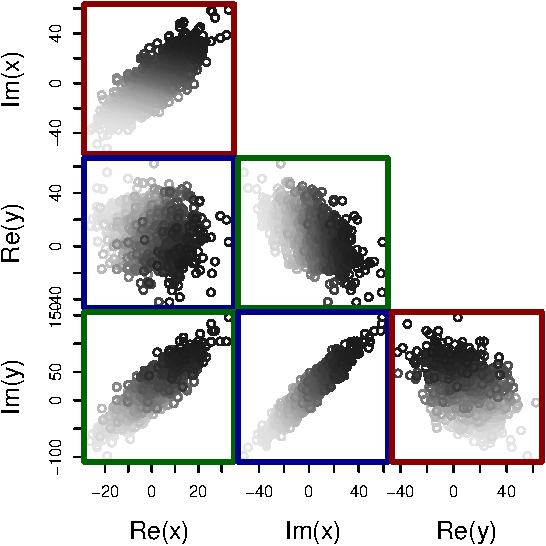
\includegraphics{Svetunkov---Svetunkov---Complex-Dynamic-Models_files/figure-latex/crvScatterplots-1.pdf}
\caption{\label{fig:crvScatterplots}Visualisation of relations between two complex variables}
\end{figure}

This scatterplot has several important elements in it:

\begin{itemize}
\tightlist
\item
  It shows relations between real and imaginary parts of each variable (e.g.~the two scatterplots in the bold dark red frame),
\item
  It shows cross-relations between parts of one variable and parts of the other one (e.g.~the rest four plots),
\item
  The colour shows ordering of the original variable \(x\) with dark values corresponding to point with higher magnitude and light ones being closer to zero. This way, we can see what the original points in \(x\) correspond to in \(y\).
\end{itemize}

The plots are positioned to satisfy two rules:

\begin{enumerate}
\def\labelenumi{\arabic{enumi}.}
\tightlist
\item
  When a scatterplot for a c.r.v. is produced, the real part should be in x-axis, while the imaginary should be in the y-axis.
\item
  When parts of variables \(x\) and \(y\) are compared, the part for \(x\) should be in x-axis, while the part for \(y\) should be in y-axis, which should the reflect the idea that \(x\) could be an explanatory variable for \(y\).
\end{enumerate}

While a simple scatterplot matrix could have been constructed instead of Figure \ref{fig:crvScatterplots}, we argue that the latter has a logical grouping and should be preferred for analysis of complex variables. For example, based on the plots in Figure \ref{fig:crvScatterplots} we can conclude that:

\begin{itemize}
\tightlist
\item
  There is a positive relation between the real and imaginary parts of \(x\),
\item
  There is a negative relation between the real and imaginary parts of \(y\),
\item
  Real parts of \(x\) and \(y\) do not exhibit a strong linear relation,
\item
  But the respective imaginary parts of \(x\) and \(y\) have the positive relation between them,
\item
  Finally, we see that with the increase of real and imaginary parts of \(x\), the real part of \(y\) decreases, while the imaginary one increases. This sort of behaviour implies positive complex slope in the potential linear regression (discussed in Section \ref{simpleCLR}).
\end{itemize}

We think that this visualisation is useful when analysing relations between two complex random variables. But it also shows how complicated it is to capture the relation between them and how many aspects need to be considered.

\hypertarget{conjugate-and-direct-correlations}{%
\subsection{Conjugate and Direct correlations}\label{conjugate-and-direct-correlations}}

The literature knows two correlation coefficients for complex variables \citep{ref}: the conjugate and the direct correlation (the latter is known in the literature as ``pseudo-correlation''). Their formula are based on the respective covariances and variances (conjugate and direct discussed in Subsection \ref{crvSecondMoment}):

\begin{enumerate}
\def\labelenumi{\arabic{enumi}.}
\item
  Conjugate correlation
  \begin{equation}
   \rho_{x,y} = \frac{\sqrt{\sigma_{x,y} \sigma_{y,x}}}{\sigma_x \sigma_y},
   \label{eq:correlationConventional}
  \end{equation}
\item
  Direct correlation
  \begin{equation}
   \varrho_{x,y} = \frac{\varsigma_{x,y}}{\varsigma_x \varsigma_y}.
   \label{eq:correlationPseudo}
  \end{equation}
\end{enumerate}

Note that the conjugate correlation has the geometric mean of standard deviations in the numerator. This is needed because of the issue with the conjugate covariance (its value changes with the change of conjugate number). The geometric mean appears from the definition of the original Pearson's correlation coefficient \citep{refPearson}. In that case, the correlation coefficient equals to the geometric mean of slopes of two regression lines:
\begin{equation}
    \begin{aligned}
        &y = \beta_0 + \beta_1 x + \epsilon \\
        &x = \alpha_0 + \alpha_1 y + \upsilon ,
    \end{aligned}
    \label{eq:twoRegressions}
\end{equation}
where \(\alpha_0\) and \(\beta_0\) are the intercepts, \(\alpha_1\) and \(\beta_1\) are the slopes of the regression lines and \(e\) and \(u\) are the residuals of the models. As we show in Section \ref{simpleCLR}, the parameters of slope can be estimated using Ordinary Least Squares (OLS) or the Complex Least Squares (CLS) to get respectively \(a_1\) and \(b_1\). For the OLS, the formulae for the slopes are:
\begin{equation}
    \begin{aligned}
        &b_1 = \frac{\hat{\sigma}_{x,y}}{\hat{\sigma}_x} \\
        &a_1 = \frac{\hat{\sigma}_{x,y}}{\hat{\sigma}_y} .
    \end{aligned}
    \label{eq:twoRegressionsOLS}
\end{equation}
Taking their geometric means leads to:
\begin{equation}
    \hat{\rho}_{x,y} = \sqrt{a_1 b_1},
    \label{eq:correlationConventionalEstimate}
\end{equation}
which then leads to the formula \eqref{eq:correlationConventional}. Similarly, for CLS estimated regressions, we have:
\begin{equation}
    \begin{aligned}
        &b_1 = \frac{\hat{\varsigma}_{x,y}}{\hat{\varsigma}_x} \\
        &a_1 = \frac{\hat{\varsigma}_{x,y}}{\hat{\varsigma}_y} ,
    \end{aligned}
    \label{eq:twoRegressionsCLS}
\end{equation}
which after taking the same geometric means leads to \eqref{eq:correlationPseudo}. Note that the estimates of the slope parameters will differ between the OLS and the CLS. This is discussed further in Section \ref{simpleCLR}.

\hypertarget{conjugate-correlation}{%
\subsection{Conjugate correlation}\label{conjugate-correlation}}

When it comes to the interpretation of the coefficients, both of them are complex numbers, but they show different things. The conjugate correlation \(\rho_{x,y}\) can be written as:
\begin{equation}
    {\rho}_{x,y} = \frac{\sigma_{x_r, y_r} + \sigma_{x_i, y_i} + i (\sigma_{x_i, y_r} - \sigma_{x_r, y_i})}{\sqrt{(\sigma_{x_r}^2 + \sigma_{x_i}^2)(\sigma_{y_r}^2 + \sigma_{y_i}^2)}} .
    \label{eq:correlationConventionalExpanded}
\end{equation}
As can be seen from the formula \eqref{eq:correlationConventionalExpanded}, the coefficient becomes a real number only when the cross-covariances between the real and imaginary parts of \(x\) and \(y\) are equal. In practice, this exotic condition can be met, when the parts for both variables are not correlated. In all the other cases, the resulting correlation coefficient will be a complex number. In general, the real part of the complex correlation \(\rho_{x,y}\) shows the average strength of linear relation between respective real and imaginary parts of two complex variables, while the imaginary part of \(\rho_{x,y}\) shows the difference between linear relations between the cross values of real and imaginary parts of \(x\) and \(y\).

The coefficient will be equal to zero, when there are no linear relations between the parts of complex variables \(x\) and \(y\). On the other hand, its real part will be close to one by absolute value if the complex relation between variables \(y\) and \(x\) is close to linear, i.e.~\(a_1 = \frac{1}{b_1}\).

In order to better understand what the real and imaginary parts of the conjugate correlation mean, we expand the formula \eqref{eq:correlationConventionalEstimate} by substituting \(b_1 = b_{1,r} + i b_{1,i}\) and \(a_1 = a_{1,r} + i a_{1,i}\):
\begin{equation}
    \begin{aligned}
        \hat{\rho}_{x,y} = & \sqrt{(a_{1,r} + i a_{1,i}) (b_{1,r}+ib_{1,i})} = \\
        & \sqrt{a_{1,r} b_{1,r} - a_{1,i} b_{1,i} + i(a_{1,r} b_{1,i} + a_{1,i} b_{1,r})},
    \end{aligned}
    \label{eq:correlationConjugateExpanded01}
\end{equation}
or in the exponential form:
\begin{equation}
    \hat{\rho}_{x,y} = R^{\frac{1}{2}} e^{i \frac{1}{2} \phi} ,
    \label{eq:correlationConjugateExpanded02}
\end{equation}
where
\begin{equation}
    \begin{aligned}
        & R = \sqrt{(a_{1,r} b_{1,r} - a_{1,i} b_{1,i})^2 + (a_{1,r} b_{1,i} + a_{1,i} b_{1,r})^2} \\
        & \phi=\arctan\left(\frac{a_{1,r} b_{1,i} + a_{1,i} b_{1,r}}{a_{1,r} b_{1,r} - a_{1,i} b_{1,i}}\right),
    \end{aligned}
    \label{eq:correlationConjugateExpanded03}
\end{equation}
As can be seen from \eqref{eq:correlationConjugateExpanded03}, there is a multitude of combinations of parameters of the model that can give the unity magnitude \(R\). For example, if \(a_{1,r} = 0.5\), \(b_{1,r} = 1\), \(a_{1,i} = -0.5\) and \(b_{1,i} = 1\), \(R\) would be equal to one. Similarly, there is a multitude of values of parameters that would give angles of \(0\), \(\frac{\pi}{2}\), \(\pi\) and \(\frac{3\pi}{2}\) leading to pure real or imaginary numbers. In fact, for the example above, \(\phi=0\), implying that the correlation coefficient will be equal to one, no matter how strong the relation between variable \(x\) and \(y\) is. This means that it is difficult to make any solid conclusions based on the conjugate correlation coefficient, but it can still be used to get some preliminary understanding of the relation.

An R example of a conjugate correlation (via \texttt{ccor()} function from \texttt{complex} package) with the aforementioned values of parameters is shown below and in Figure \ref{fig:crvCorConjugate}.

\begin{Shaded}
\begin{Highlighting}[]
\CommentTok{\# Create a c.r.v. x}
\NormalTok{x }\OtherTok{\textless{}{-}} \FunctionTok{complex}\NormalTok{(}\AttributeTok{real=}\FunctionTok{rnorm}\NormalTok{(}\DecValTok{1000}\NormalTok{,}\DecValTok{0}\NormalTok{,}\DecValTok{10}\NormalTok{), }\AttributeTok{imaginary=}\FunctionTok{rnorm}\NormalTok{(}\DecValTok{1000}\NormalTok{,}\DecValTok{0}\NormalTok{,}\DecValTok{10}\NormalTok{))}
\CommentTok{\# Create a c.r.v. y}
\NormalTok{y }\OtherTok{\textless{}{-}}\NormalTok{ (}\DecValTok{10} \SpecialCharTok{+}\NormalTok{ 15i) }\SpecialCharTok{+}\NormalTok{ (}\DecValTok{1} \SpecialCharTok{+}\NormalTok{ 1i) }\SpecialCharTok{*}\NormalTok{ x }\SpecialCharTok{+}
    \FunctionTok{complex}\NormalTok{(}\AttributeTok{real=}\FunctionTok{rnorm}\NormalTok{(}\DecValTok{1000}\NormalTok{,}\DecValTok{0}\NormalTok{,}\DecValTok{1}\NormalTok{), }\AttributeTok{imaginary=}\FunctionTok{rnorm}\NormalTok{(}\DecValTok{1000}\NormalTok{,}\DecValTok{0}\NormalTok{,}\DecValTok{1}\NormalTok{))}
\CommentTok{\# Produce the plot}
\FunctionTok{cplot}\NormalTok{(x, y)}
\end{Highlighting}
\end{Shaded}

\begin{figure}
\centering
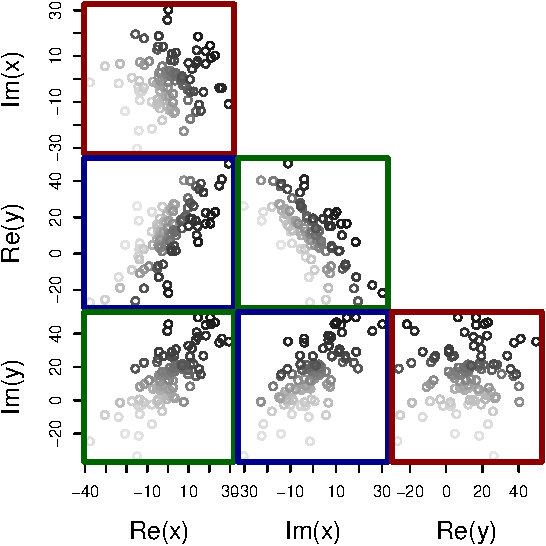
\includegraphics{Svetunkov---Svetunkov---Complex-Dynamic-Models_files/figure-latex/crvCorConjugate-1.pdf}
\caption{\label{fig:crvCorConjugate}Visualisation of relations between two complex variables}
\end{figure}

\begin{Shaded}
\begin{Highlighting}[]
\CommentTok{\# Conjugate correlation}
\FunctionTok{ccor}\NormalTok{(x, y, }\AttributeTok{kind=}\StringTok{"conjugate"}\NormalTok{)}
\end{Highlighting}
\end{Shaded}

\begin{verbatim}
## [1] 0.99745+0i
\end{verbatim}

As can be seen from the Figure \ref{fig:crvCorConjugate} and the value of the conjugate correlation, there is a relation between the two complex variables \(x\) and \(y\), but it although the value of the latter is approximately 0.997+0i, we cannot conclude unambiguously that the relation is strong.

\hypertarget{direct-correlations}{%
\subsection{Direct correlations}\label{direct-correlations}}

The direct correlation can be expanded to:
\begin{equation}
    {\varrho}_{x,y} = \frac{\sigma_{x_r, y_r} - \sigma_{x_i, y_i} + i (\sigma_{x_i, y_r} + \sigma_{x_r, y_i})}{\sqrt{(\sigma_{x_r}^2 - \sigma_{x_i}^2 + i2 \sigma_{x_r,x_i})(\sigma_{y_r}^2 - \sigma_{y_i}^2 + i2 \sigma_{y_r,y_i})}}.
    \label{eq:correlationPseudoExpanded}
\end{equation}
Given that it contains a complex number in the denominator, it is more complicated than the conjugate one.

Father's stuff here.

To get other insights about the direct correlation coefficient, we express its denominator in the exponential form:
\begin{equation}
    {\sqrt{(\sigma_{x_r}^2 - \sigma_{x_i}^2 + i2 \sigma_{x_r,x_i})(\sigma_{y_r}^2 - \sigma_{y_i}^2 + i2 \sigma_{y_r,y_i})}} = R_1^{\frac{1}{2}} e^{i \frac{\phi_1}{2}},
    \label{eq:correlationPseudoExpandedExp01}
\end{equation}
where \(R_1 = \sqrt{\left((\sigma_{x_r}^2 - \sigma_{x_i}^2)(\sigma_{y_r}^2 - \sigma_{y_i}^2) - 4 \sigma_{x_r,x_i} \sigma_{y_r,y_i} \right)^2+ 4 \left( (\sigma_{x_r}^2 - \sigma_{x_i}^2) \sigma_{y_r,y_i} + (\sigma_{y_r}^2 - \sigma_{y_i}^2) \sigma_{x_r,x_i} \right)^2}\) and \(\phi_1=\arctan \left(\frac{2 \left( (\sigma_{x_r}^2 - \sigma_{x_i}^2) \sigma_{y_r,y_i} + (\sigma_{y_r}^2 - \sigma_{y_i}^2) \sigma_{x_r,x_i} \right)}{(\sigma_{x_r}^2 - \sigma_{x_i}^2)(\sigma_{y_r}^2 - \sigma_{y_i}^2) - 4 \sigma_{x_r,x_i} \sigma_{y_r,y_i}}\right)\), which are obtained by opening the brackets inside the square root. If we now insert \eqref{eq:correlationPseudoExpandedExp01} in \eqref{eq:correlationPseudoExpanded} and multiply both numerator and denominator by conjugate number to the \eqref{eq:correlationPseudoExpandedExp01} we will get:
\begin{equation}
    {\varrho}_{x,y} = \frac{\left(\sigma_{x_r, y_r} - \sigma_{x_i, y_i} + i (\sigma_{x_i, y_r} + \sigma_{x_r, y_i})\right)e^{-i \frac{\phi_1}{2}}}{R_1^{\frac{1}{2}}}.
    \label{eq:correlationPseudoExpandedExp02}
\end{equation}
Representing the \(\sigma_{x_r, y_r} - \sigma_{x_i, y_i} + i (\sigma_{x_i, y_r} + \sigma_{x_r, y_i})\) as \(R_2 e^{i \phi_2}\), where \(R_2= \sqrt{(\sigma_{x_r, y_r} - \sigma_{x_i, y_i})^2 + (\sigma_{x_i, y_r} + \sigma_{x_r, y_i})^2}\) and \(\phi_2= \arctan \left( \frac{\sigma_{x_i, y_r} + \sigma_{x_r, y_i}}{\sigma_{x_r, y_r} - \sigma_{x_i, y_i}} \right)\), and inserting these values in \eqref{eq:correlationPseudoExpandedExp02} we get:
\begin{equation}
    {\varrho}_{x,y} = \frac{R_2}{\sqrt{R_1}} e^{i \left(\phi_2 - \frac{\phi_1}{2} \right)}.
    \label{eq:correlationPseudoExpandedExp03}
\end{equation}
or in an even shorter exponential form \({\varrho}_{x,y} = |{\varrho}_{x,y}| e ^{i \arg({\varrho}_{x,y})}\), where:
\begin{equation}
    |{\varrho}_{x,y}|=\sqrt{\frac{(\sigma_{x_r, y_r} - \sigma_{x_i, y_i})^2 +  (\sigma_{x_i, y_r} + \sigma_{x_r, y_i})^2}{\sqrt{\left((\sigma_{x_r}^2 - \sigma_{x_i}^2)(\sigma_{y_r}^2 - \sigma_{y_i}^2) - 4 \sigma_{x_r,x_i} \sigma_{y_r,y_i} \right)^2+ 4 \left( (\sigma_{x_r}^2 - \sigma_{x_i}^2) \sigma_{y_r,y_i} + (\sigma_{y_r}^2 - \sigma_{y_i}^2) \sigma_{x_r,x_i} \right)^2}}}
    \label{eq:correlationPseudoExpandedExpR}
\end{equation}
and
\begin{equation}
    \arg({\varrho}_{x,y}) = \arctan \left( \frac{\sigma_{x_i, y_r} + \sigma_{x_r, y_i}}{\sigma_{x_r, y_r} - \sigma_{x_i, y_i}} \right) - \frac{1}{2}\arctan \left(\frac{2 \left( (\sigma_{x_r}^2 - \sigma_{x_i}^2) \sigma_{y_r,y_i} + (\sigma_{y_r}^2 - \sigma_{y_i}^2) \sigma_{x_r,x_i} \right)}{(\sigma_{x_r}^2 - \sigma_{x_i}^2)(\sigma_{y_r}^2 - \sigma_{y_i}^2) - 4 \sigma_{x_r,x_i} \sigma_{y_r,y_i}}\right) .
    \label{eq:correlationPseudoExpandedExpPhi}
\end{equation}
Analysing \eqref{eq:correlationPseudoExpandedExpR} \eqref{eq:correlationPseudoExpandedExpPhi}, we can identify several conditions that lead to specific values of the direct correlation coefficient:

\begin{enumerate}
\def\labelenumi{\arabic{enumi}.}
\item
  The magnitude of the coefficient will be equal to zero (and thus the coefficient will be equal to zero) only when \(\sigma_{x_i,y_r}=\sigma_{x_r,y_i}=0\) and \(\sigma_{x_r,y_r}=\sigma_{x_i,y_i}\). One of the special cases of this is when all cross-covariances between the real and imaginary parts of \(x\) and \(y\) are equal to zero.
\item
  The magnitude of the coefficient will be equal to one, when its numerator and denominator are equal, which can be obtained with a multitude of values of covariances and variances of real and imaginary parts of complex variables \(x\) and \(y\).
\item
  One of the special cases for \(\varrho_{x,y}=1\) comes to the definition of the conventional correlation coefficient \citep{refPearson}. \(\sqrt{a_1 b_1}=1\)
\end{enumerate}

\hypertarget{simpleCLR}{%
\section{Simple CLR}\label{simpleCLR}}

\hypertarget{model-formulation}{%
\subsection{Model formulation}\label{model-formulation}}

The simple Complex Linear Regression can be written as:
\begin{equation}
    \mathbf{z} = \mathbf{a} + \mathbf{b} \mathbf{x} + \boldsymbol{\epsilon}
    \label{eq:SimpleCLRComplex}
\end{equation}
or
\begin{equation}
    y_r + i y_i = a_0 + i a_1 + (b_0 + i b_1) (x_r + i x_i) + \epsilon_r + i \epsilon_i
    \label{eq:SimpleCLR}
\end{equation}
Given that any complex equation can be represented as a system of two equations, this model can be represented as a system of two linear regressions:
\begin{equation}
    \begin{aligned}
        y_r = & a_0 + b_0 x_r - b_1 x_i + \epsilon_r \\
        y_i = & a_1 + b_0 x_i + b_1 x_r + \epsilon_i
    \end{aligned}
    \label{eq:SimpleCLRSystem}
\end{equation}
This model captures a very specific dynamics between the real and imaginary parts, given that they share the same set of parameters for the slope.

\hypertarget{estimation}{%
\subsection{Estimation}\label{estimation}}

Number of estimated parameters is k, number of degrees of freedom per series is k/2.

\hypertarget{inference}{%
\subsection{Inference}\label{inference}}

\hypertarget{forecasting}{%
\subsection{Forecasting}\label{forecasting}}

\hypertarget{multiple-clr}{%
\section{Multiple CLR}\label{multiple-clr}}

\hypertarget{model-formulation-1}{%
\subsection{Model formulation}\label{model-formulation-1}}

\hypertarget{estimation-1}{%
\subsection{Estimation}\label{estimation-1}}

\hypertarget{inference-1}{%
\subsection{Inference}\label{inference-1}}

\hypertarget{diagnostics}{%
\subsection{Diagnostics}\label{diagnostics}}

\hypertarget{forecasting-1}{%
\subsection{Forecasting}\label{forecasting-1}}

\hypertarget{examples-of-application-production-functions}{%
\subsection{Examples of application (Production functions)}\label{examples-of-application-production-functions}}

  \bibliography{library.bib,packages.bib,websites.bib}

\end{document}
